\question{1}{<Short question title>}{<Restate the question here.>}

\begin{parambox}
  \begin{tabular}{@{}ll@{}}
    $a$ & <value with unit> \\
  \end{tabular}
\end{parambox}

\subsection*{Setup}
<What is given and what is being asked.>

\subsection*{Step 1 -- <first step>}
\begin{equation}
  D = \frac{k_B T}{6 \pi \eta a}
  \label{eq:stokes-q1}
\end{equation}
where <define the symbols>.

\subsection*{Step 2 -- <second step>}
<Continue. Reference equation~\eqref{eq:stokes-q1} instead of repeating it.>

\begin{answerbox}
  \[
    t = \frac{\mean{x^2}}{2D}
  \]
\end{answerbox}

\subsection*{Discussion}
<Physical reading of the result.>

\begin{figure}[H]
  \centering
  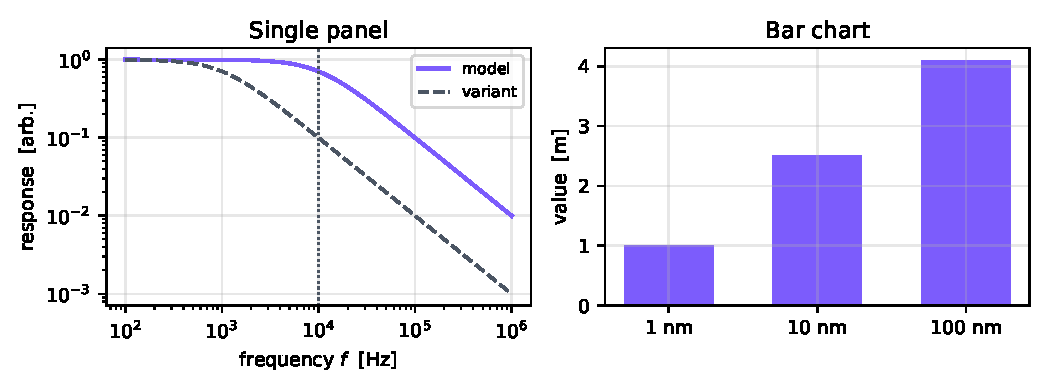
\includegraphics[width=0.9\textwidth]{fig/example.pdf}
  \caption{<What the figure shows.>}
  \label{fig:example-q1}
\end{figure}
